% -*- latex -*-
%%%%%%%%%%%%%%%%%%%%%%%%%%%%%%%%%%%%%%%%%%%%%%%%%%%%%%%%%%%%%%%%
%%%%%%%%%%%%%%%%%%%%%%%%%%%%%%%%%%%%%%%%%%%%%%%%%%%%%%%%%%%%%%%%
%%%%
%%%% This text file is part of the source of slides for
%%%% `Introduction to High-Performance Scientific Computing'
%%%% by Victor Eijkhout, copyright 2012-2022
%%%%
%%%%%%%%%%%%%%%%%%%%%%%%%%%%%%%%%%%%%%%%%%%%%%%%%%%%%%%%%%%%%%%%
%%%%%%%%%%%%%%%%%%%%%%%%%%%%%%%%%%%%%%%%%%%%%%%%%%%%%%%%%%%%%%%%

\Level 1 {Incomplete approaches to matrix factorization}

\frame[containsverbatim]{\frametitle{Sparse operations in parallel: mvp}
Mvp $y=Ax$
\begin{verbatim}
  for i=1..n
    y[i] = sum over j=1..n a[i,j]*x[j]
\end{verbatim}
In parallel:
\begin{verbatim}
  for i=myfirstrow..mylastrow
    y[i] = sum over j=1..n a[i,j]*x[j]
\end{verbatim}
}

\frame[containsverbatim]{\frametitle{How about ILU solve?}
Consider $Lx=y$
\begin{verbatim}
  for i=1..n
    x[i] = (y[i] - sum over j=1..i-1 ell[i,j]*x[j]) 
           / a[i,i]
\end{verbatim}
Parallel code:
\begin{verbatim}
  for i=myfirstrow..mylastrow
    x[i] = (y[i] - sum over j=1..i-1 ell[i,j]*x[j]) 
           / a[i,i]
\end{verbatim}
Problems?
}

\frame[containsverbatim]{\frametitle{Block method}
\begin{verbatim}
  for i=myfirstrow..mylastrow
    x[i] = (y[i] - sum over j=myfirstrow..i-1 ell[i,j]*x[j]) 
           / a[i,i]
\end{verbatim}
Block Jacobi with local GS solve
}

\frame{\frametitle{}
\begin{figure}[ht]
  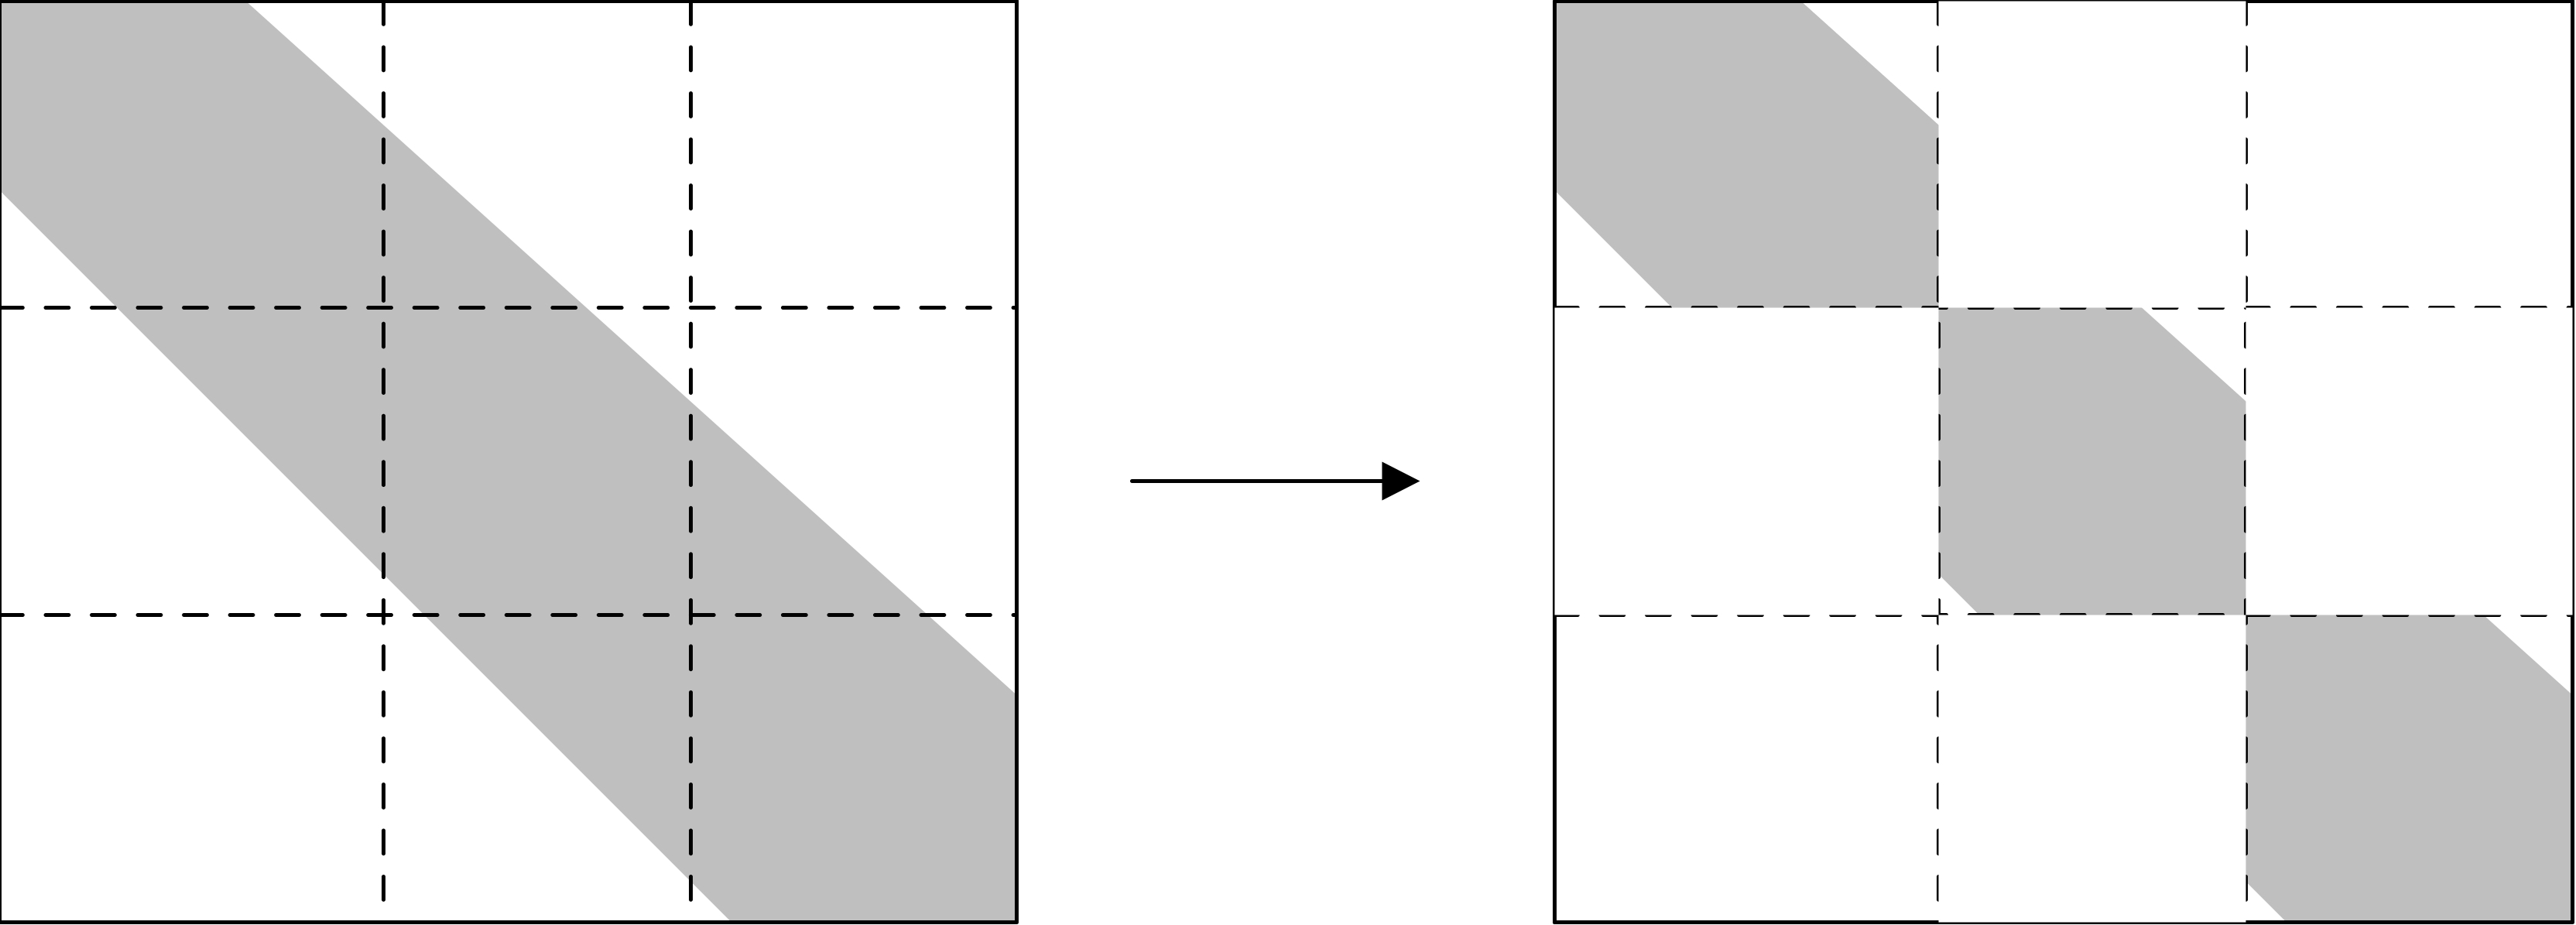
\includegraphics[scale=.12]{block-jacobi}
  \caption{Sparsity pattern corresponding to a block Jacobi
    preconditioner.}
  \label{fig:block-method}
\end{figure}
}

\frame{\frametitle{Variable reordering}
\footnotesize
\[ 
\begin{pmatrix}
  a_{11}&a_{12}&&&&\emptyset\\ a_{21}&a_{22}&a_{23}\\ 
  &a_{32}&a_{33}&a_{34}\\ \emptyset&&\ddots&\ddots&\ddots
\end{pmatrix}
\begin{pmatrix}  x_1\\ x_2\\ x_3\\ \vdots\end{pmatrix} =
\begin{pmatrix}  y_1\\ y_2\\ y_3\\ \vdots\end{pmatrix}
\]
with redblack
\[ 
\begin{pmatrix}
  a_{11}&&&&a_{12}\\ &a_{33}&&&a_{32}&a_{34}\\ &&a_{55}&&&\ddots&\ddots\\
  &&&\ddots\\
  a_{21}&a_{23}&&&a_{22}\\ &a_{43}&a_{45}&&&a_{44}\\ &&\ddots&\ddots&&&\ddots
\end{pmatrix}
\begin{pmatrix}  x_1\\ x_3\\ x_5\\ \vdots\\ x_2\\ x_4\\ \vdots\end{pmatrix} =
\begin{pmatrix}  y_1\\ y_3\\ y_5\\ \vdots\\ y_2\\ y_4\\ \vdots\end{pmatrix}
\]
Two-processor parallel Gauss-Seidel or ILU
}

\frame{\frametitle{2D redblack}
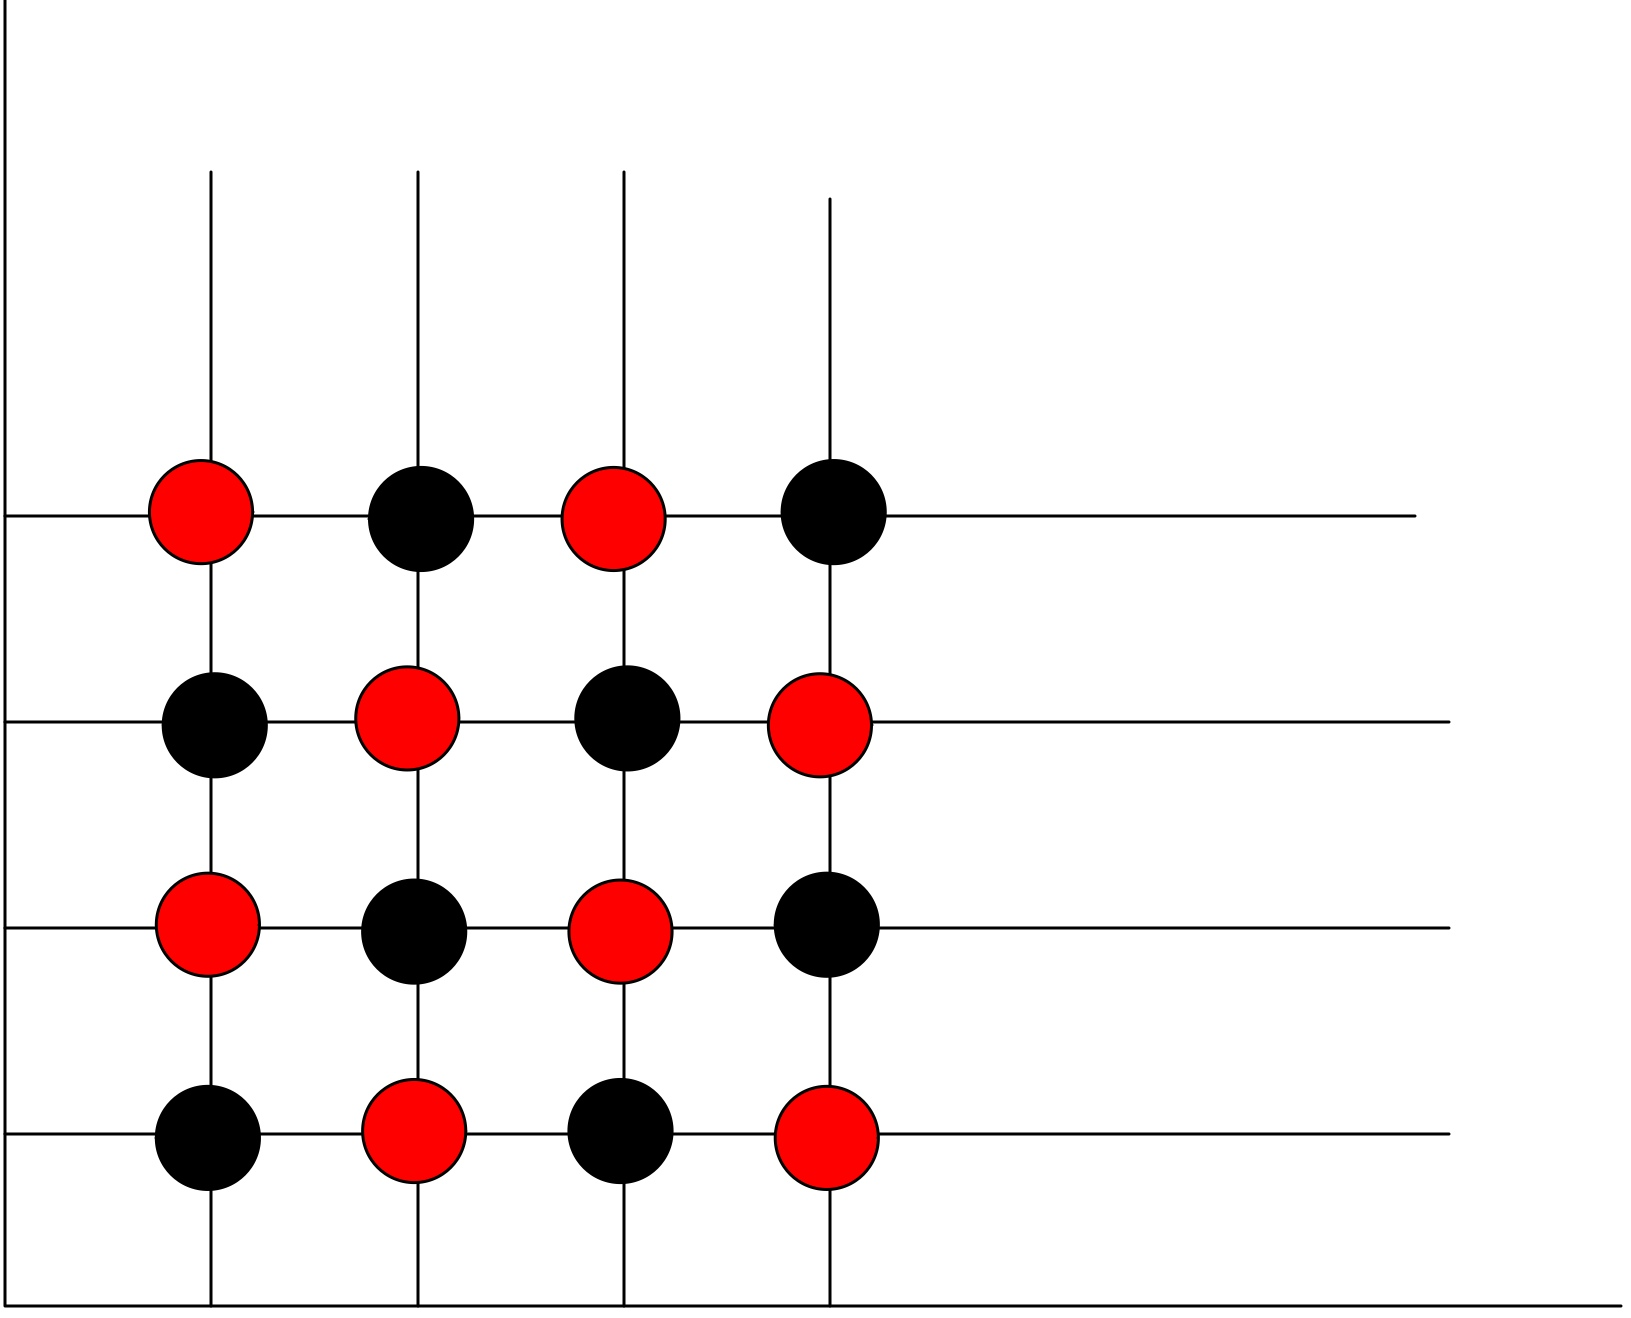
\includegraphics[scale=.1]{redblack}

In general, colouring, colour number
}

\frame{\frametitle{Multicolour ILU}
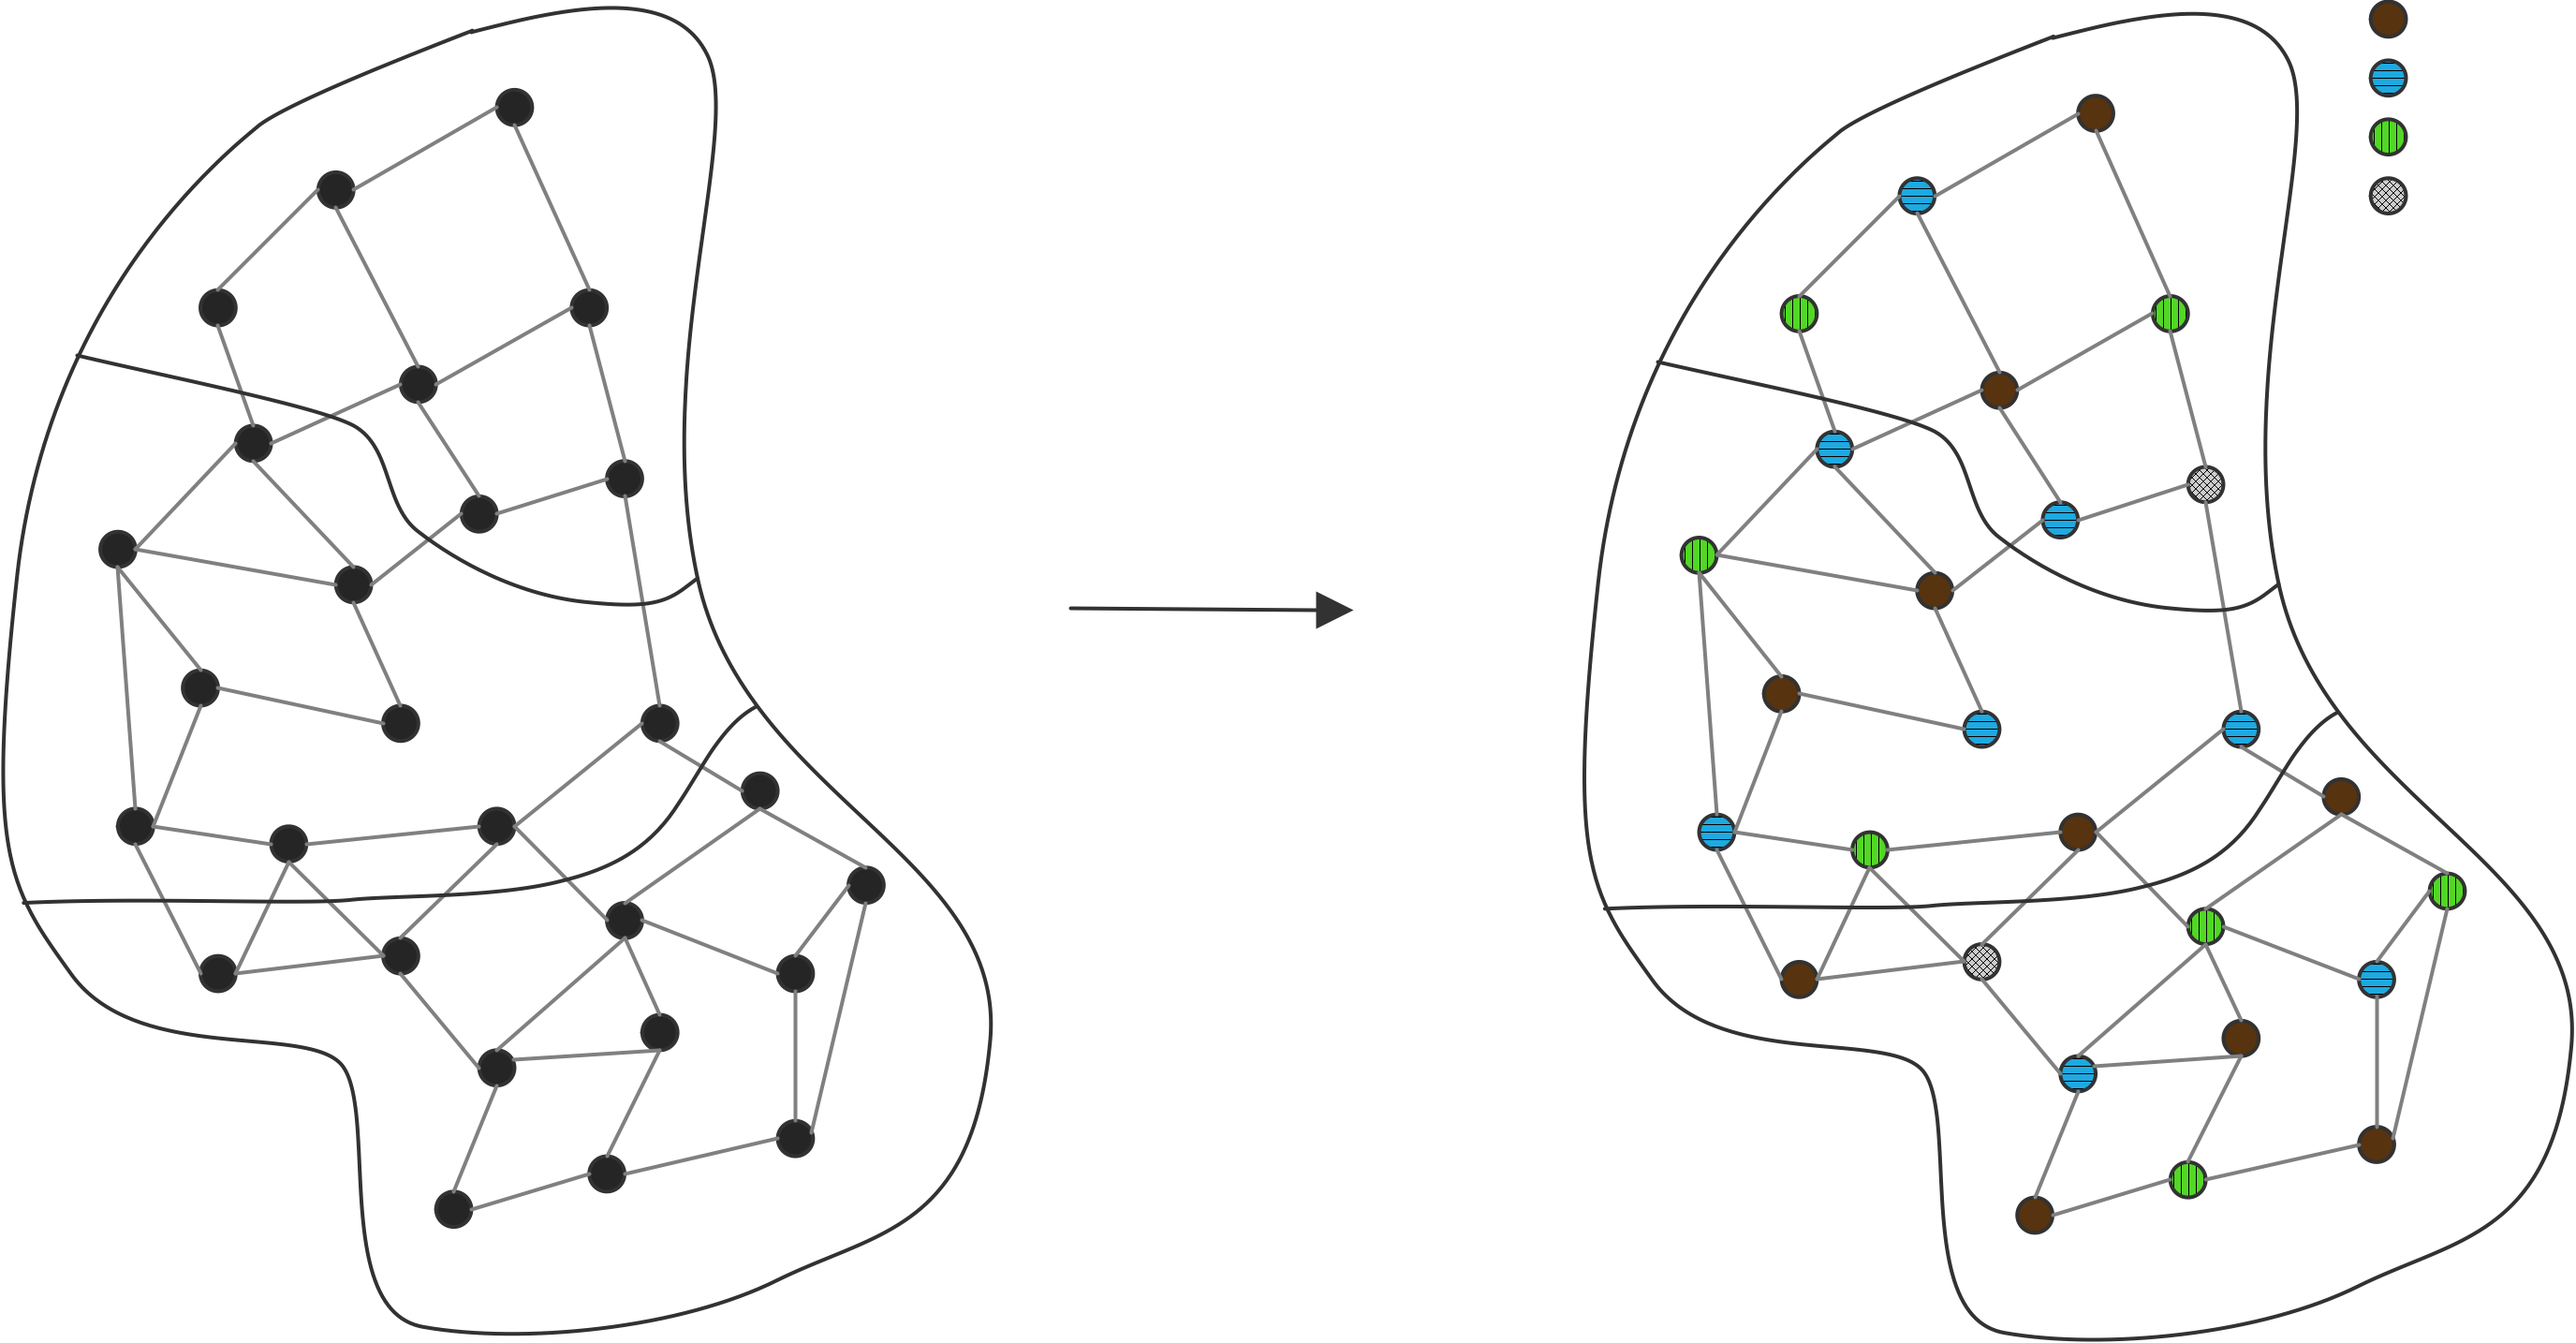
\includegraphics[scale=.1]{pilu}
}
\frame{\frametitle{}
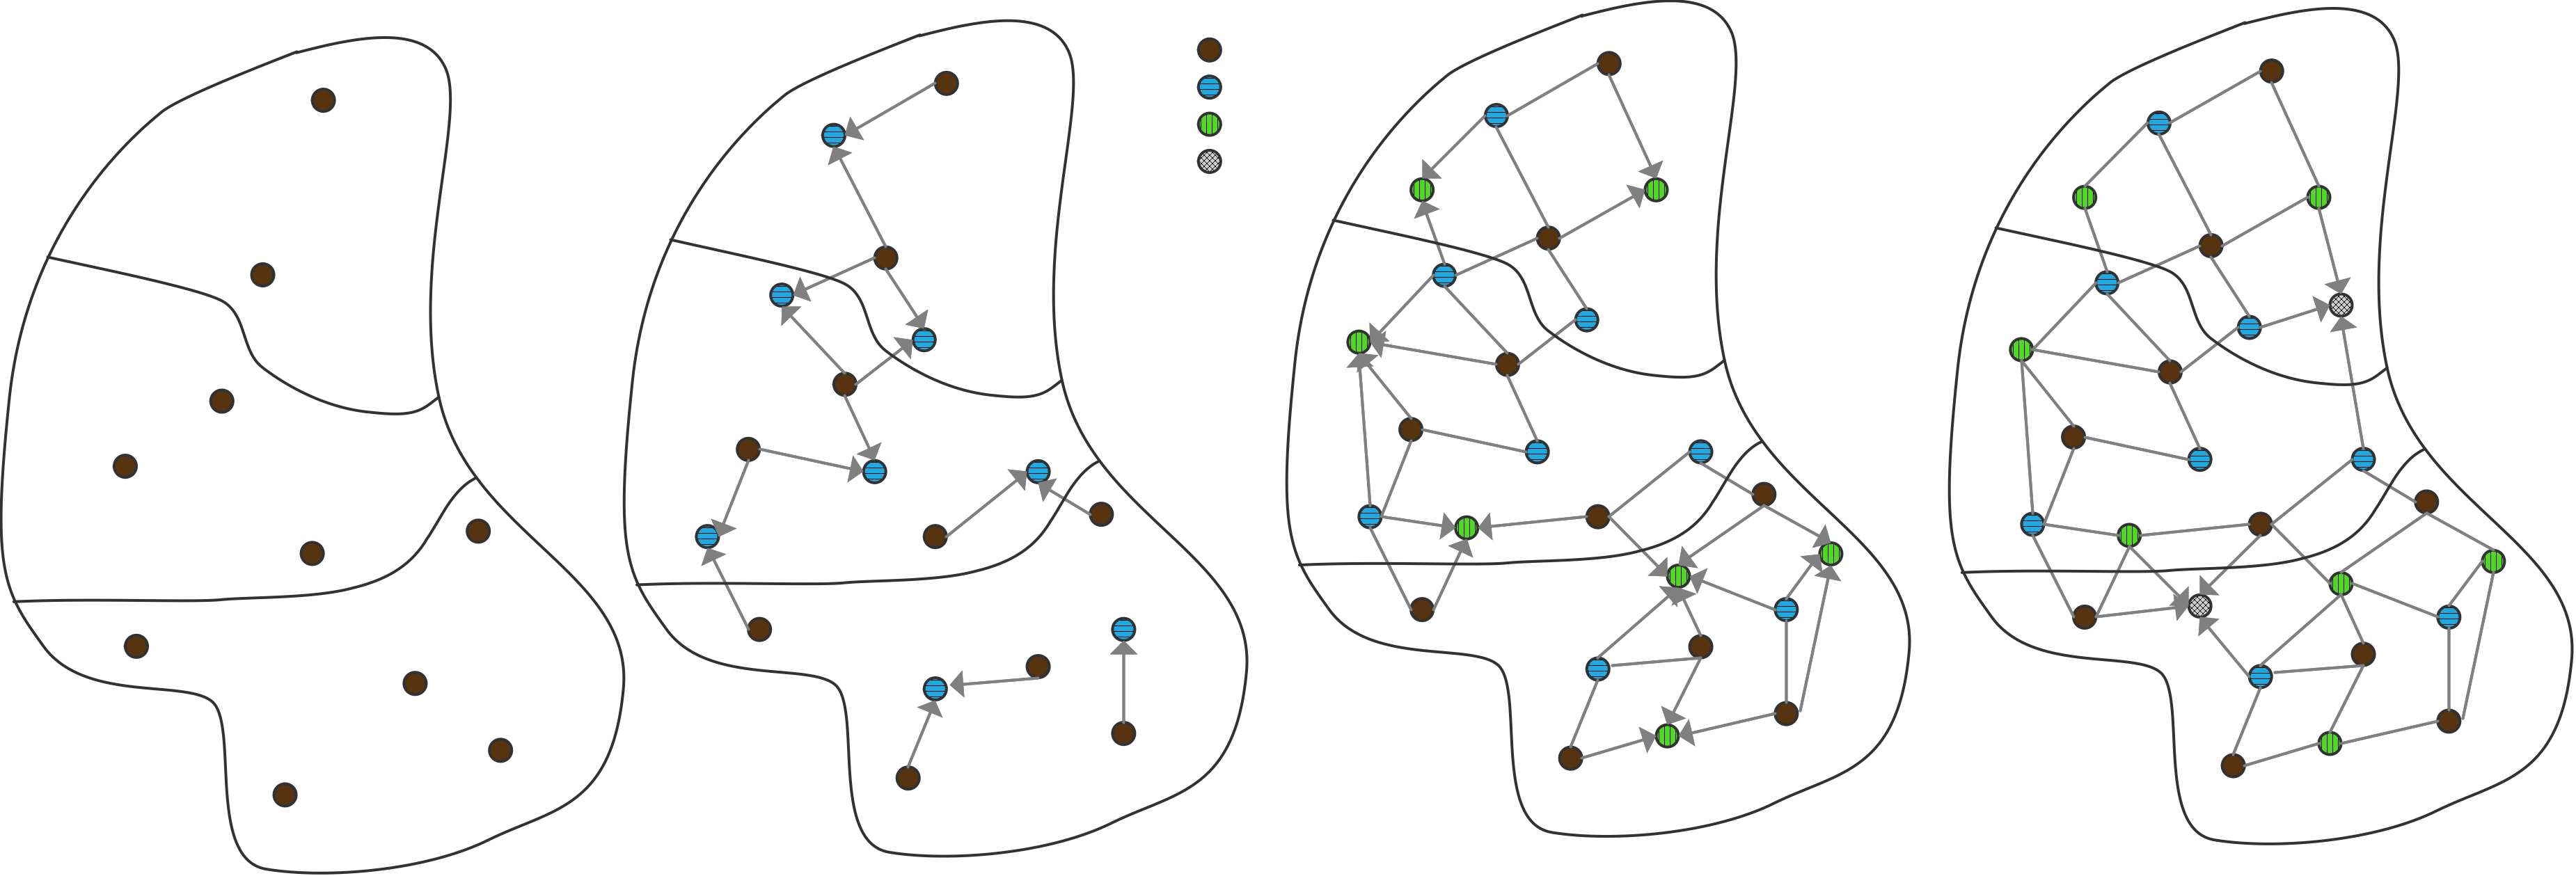
\includegraphics[scale=.1]{pilu-solve}
}

\begin{frame}{How do you get a multi-colouring?}
  Exactly colour number is NP-completely: don't bother.

  For preconditioner an approximation is good enough:\\
  Luby / Jones-Plassman algorithm
  \begin{itemize}
  \item Give every node a random value
  \item First colour: all nodes with a higher value than all their neighbours
  \item Second colour: higher value than all neighbours except in first colour
  \item et cetera
  \end{itemize}
\end{frame}

